% -*- TeX:de -*-
\NeedsTeXFormat{LaTeX2e}
\documentclass[12pt,a4paper,titlepage]{article}

\usepackage[german]{babel} % german text
\usepackage[DIV12]{typearea} % size of printable area
\usepackage[T1]{fontenc} % font encoding
\usepackage[utf8]{inputenc} % probably on Linux

\usepackage{graphicx} % to include images
\usepackage{subfigure} % for creating subfigures
\usepackage{amsmath} % a bunch of symbols
\usepackage{amssymb} % even more symbols
\usepackage{booktabs} % pretty tables
\usepackage{csquotes}

% a floating environment for circuits
\usepackage{float}
\usepackage{caption}

\usepackage[european]{circuitikz}
\ctikzset{voltage/distance from line=.25}% pos. between 0 and 1

\newfloat{circuit}{tbph}{circuits}
\floatname{circuit}{Schaltplan}

% a floating environment for diagrams
\newfloat{diagram}{tbph}{diagrams}
\floatname{diagram}{Diagramm}

\renewcommand{\familydefault}{\sfdefault} % activate to use sans-serif font as default

\sloppy % friendly typesetting

\usepackage{eurosym}
\usepackage{makeidx}
\usepackage{amsfonts}
\usepackage{mparhack}
\usepackage{array}
\usepackage{tabularx}
\usepackage{minitoc}
\usepackage[colorlinks=true]{hyperref}
\usepackage{epstopdf}
\usepackage{setspace}
\usepackage{csquotes}

\usepackage{pgfplots}

\begin{document}

\begin{titlepage}

\begin{figure*}[h!]
  
\includegraphics[width=8cm]{TULogo_CMYK}
\end{figure*}

\begin{center}
\vspace*{1.3cm}
{\Huge Elektrotechnische Grundlagen der Informatik\\(LU 182.692)\\}
\vspace{1.7cm}
{\LARGE Protokoll der 2. Laborübung: \enquote{Filter}\\}
{\large \enquote{Transiente Vorgänge und Frequenzverhalten}\\}
{\LARGE b) Messungen\\}
\vspace{1.5cm}

% fill in group number and date of lab here
% CHANGE ME!
{\Large Gruppennr.: 10 \hspace{1cm} Datum der Laborübung: 19.05.2017}

% fill in IDs and names here
% CHANGE ME!
\begin{table}[h!]
\centering
\begin{tabular}{|p{3.5cm}|p{3.5cm}|p{6.5cm}|}
\hline \textbf{Matr. Nr.} & \textbf{Kennzahl} & \textbf{Name} \\
\hline
1609418 & 033 535 & GEISELBRECHTINGER Max \\
\hline
1625753 & 033 535 & HAAR Martin \\
\hline
& & \\
\hline
\end{tabular}
\end{table}

\end{center}
\vspace{1.0cm}

\begin{table}[h!]
\begin{tabular}{|l|l|}
\hline \textbf{Kontrolle} & \checkmark \\
\hline Verhalten eines Filters 1. Ordnung & \\
\hline Verhalten eines RL-Filters & \\
\hline Dynamisches System 2. Ordnung & \\
\hline
\end{tabular}
\end{table}

\end{titlepage}
\setcounter{page}{2}

% start of actual lab protocol
% CHANGE ME!
% !TEX root = deckblatt2b.tex

\section{RC-Tiefpass}

\begin{figure}[H]
  \begin{center}
    %\tikzset{component/.style={draw,thick,circle,fill=white,minimum size =0.75cm,inner sep=0pt}}
    \begin{circuitikz}
      \draw (0,2)
      to[R=$R$] (3,2)
      to[short] (6,2);
      \draw (4,2)
      to[C=$C$] (4,0);
      \draw (0,0)
      to[short] (6,0);
      \draw (0,1.8)
       to[short] (0,0.7) node[vee] {};
      \draw (-0.5,1) node[] {$U_e$};
      \draw (6,1.8)
       to[short] (6,0.7) node[vee] {};
      \draw (6.5,1) node[] {$U_a$};
    \end{circuitikz}
    \caption{RC-Tiefpass 1.Ordnung}
    \vspace{1cm}
    Das Schaltbild zeigt den Messaufbau des RC-Tiefpassfilters 1.Ordnung.\\
    $R=22k\Omega, C=1nF, U_e=1V$\\
  \end{center}
\end{figure}

\subsection{Sprungantwort}
\begin{figure}[H]
 \begin{center}
  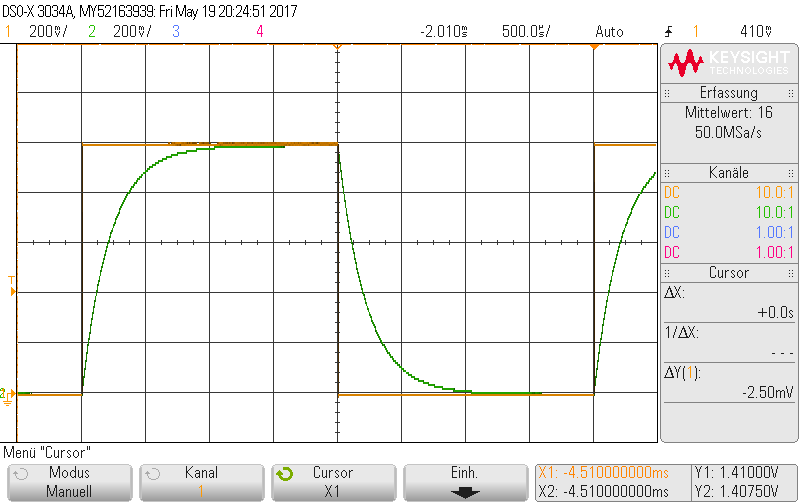
\includegraphics[height=6cm,width=12cm]{Oszi_Bilder/RC_Sprung}
 \end{center}
 \caption{Sprungantwort RC-Tiefpass}
\end{figure}
\noindent
In der Abbildung der Sprungantwort sind die exponentiellen Lade- und Entladekurven des Kondesators zu sehen. \\
\begin{align*}
 U_{charge} &= U_e(1 - e^{-\frac{t}{\tau}})\\
 U_{drain} &= U_e e^{-\frac{t}{\tau}}\\
 \tau &= RC
\end{align*}
\noindent
Die Zeitkonstante kann direkt aus der Sprungantwort abgelesen werden, indem man die Zeitdifferenz von $U_e=0$ bis $U_C \approx 0,6U_e$ misst. Daraus ergibt
sich ein $\tau_{gemessen}$ von $210\mu s$, dass gegenüber einem $\tau_{berechnet}$ von $220\mu s$ steht. Der Messfehler ergibt sich durch, ungenaues ablesen
ablesen mit dem Cursor und Bauteiltoleranzen.\\

\subsection{Bode Diagramm}

Das Bode Diagramm zeigt den Verlauf der Dämpfung und des Phasenwinkels des Filters in abhängigkeit der Frequenz.\\
\begin{figure}[H]
  \centering
  \begin{tikzpicture}
    \begin{axis}[width=15cm, height=7cm, xmode=log, xmin=10, xmax=1e7, xlabel={$Hz$}, ylabel={dB},y tick label style={grid=major}]
      \addplot table[x=Frequenz, y=dB, col sep=comma] {csv_files/RC_dB.csv};
      \node[label={260:{$f_g$}},square,fill=blue,inner sep=3pt] at (axis cs:723.43,-3) {};
    \end{axis}
  \end{tikzpicture}
  \caption{Bode Diagramm RC-Tiefpass, Dämpfung}
\end{figure}
\noindent
Die niedrigen Frequenzen werden vom Tiefpassfilter ungedämpft durchgelassen. Erst ab der Grenzfrequenz, von $f_g = \frac{1}{2\pi RC} = 723,43Hz$, nimmt die Dämpfung
mit $-20dB/DEK$ zu. Ab $100kHz$ war die Dämpfung mit dem Oszilloskop nahezu nicht mehr messbar. \\

\begin{figure}[H]
  \centering
  \begin{tikzpicture}
    \begin{axis}[width=15cm, height=7cm, xmode=log, xmin=10, xmax=1e7, xlabel={$Hz$}, ylabel={$\phi$},y tick label style={grid=major}]
      \addplot table[x=Frequenz, y=Phi, col sep=comma] {csv_files/RC_Phi.csv};
      \node[label={260:{$f_g$}},square,fill=blue,inner sep=3pt] at (axis cs:723.43,-45) {};
    \end{axis}
  \end{tikzpicture}
  \caption{Bode Diagramm RC-Tiefpass, Phasengang}
\end{figure}
\noindent
Der Phasengang verläuft von $0^\circ$ bis $-90^\circ$. Auch hier wurde die Messung ab $100kHz$ sehr ungenau. Die Grenzfrequenz liegt hier bei $-45^\circ$.\\
\\
Die Messergebnisse des RC-Tiefpassfilters 1.Ordnung stimmen, bis auf kleine Abweichungen durch Messfehler und Bauteiltoleranzen, weitest gehend mit der Simmulation überein. 
Nur bei hohen Frequenzen, ab ca $100kHz$, gab es bei der Messung der Ausgangsspannung und des Phasenwinkels ungenauigkeiten, auf Grund der fortgeschrittenen Dämpfung war das
Ausgangssignal kaum mehr zu messen. \\
% !TEX root = deckblatt2b.tex

\section{RL-Hochpass}
\begin{figure}[H]
  \begin{center}
    %\tikzset{component/.style={draw,thick,circle,fill=white,minimum size =0.75cm,inner sep=0pt}}
    \begin{circuitikz}
      \draw (0,2)
      to[R=$47\Omega$] (3,2)
      to[short] (6,2);
      \draw (4,2)
      to[L=$1mH$] (4,0);
      \draw (0,0)
      to[short] (6,0);
      \draw (0,1.8)
       to[short] (0,0.7) node[vee] {};
      \draw (-0.5,1) node[] {$U_e=1V$};
      \draw (6,1.8)
       to[short] (6,0.7) node[vee] {};
      \draw (6.5,1) node[] {$U_a$};
    \end{circuitikz}
    \caption{RL-Hochpass 1.Ordnung}
    \vspace{0.5cm}
    Das Schaltbild zeigt den Messaufbau des RL-Hochpassfilters 1.Ordnung.
  \end{center}
\end{figure}

\subsection{Sprungantwort}
\begin{figure}[H]
 \begin{center}
  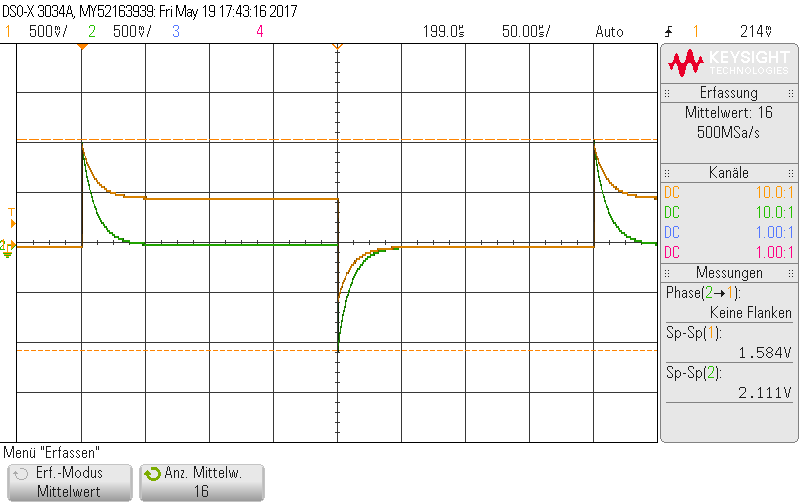
\includegraphics[height=6cm,width=12cm]{Oszi_Bilder/RL_Sprung}
 \end{center}
 \caption{Sprungantwort RL-Hochpass, $U_e$ (gelb), $U_a$ (gr\"un)}
\end{figure}
\noindent
In dieser Abbildung (Abb. 6) sind die Aus- und Einschaltvorgänge an der Spule zu sehen.
\begin{longtable}{p{0.4\textwidth}p{0.3\textwidth}p{0.3\textwidth}}
\centering
$U_{charge} = U_e e^{-\frac{t}{\tau}}$ & $U_{drain} = -U_e e^{-\frac{t}{\tau}}$ & $\tau = \frac{L}{R}$
\end{longtable}
\noindent
Die Eingangsspannung beträgt hier weniger als $0,5V$, da der Frequenzgenerator eine Spannungsquelle ist und den durch die Spule verursachten Stromfluss
nicht genügen kann. Die Induktivität der Spule ist auch verantwortlich für die Ausschläge beim Einschalten der Eingangsspannung. \\
Die Zeitkonstante kann aus der Sprungantwort abgelesen werden, indem man die Zeitdifferenz von $U_e=0$ bis $U_L \approx 0,3U_e$ misst. Daraus ergibt
sich ein $\tau_{gemessen}$ von $23\mu s$, dass gegenüber einem $\tau_{berechnet}$ von $21,28\mu s$ steht. Der Messfehler entsteht dabei, durch ungenauigkeiten
beim Ablesen mit dem Cursor und Bauteiltoleranzen.

\subsection{Bode Diagramm}
Das Bode Diagramm zeigt den Verlauf der Amplitude und des Phasenwinkels des Filters in abhängigkeit der Frequenz.
\begin{figure}[H]
  \centering
  \begin{tikzpicture}
    \begin{axis}[width=15cm, height=7cm, xmode=log, xmin=10, xmax=1e7, xlabel={Frequenz [Hz]}, ylabel={Amplitude[dB]},y tick label style={grid=major}]
      \addplot table[x=Frequenz, y=dB, col sep=comma] {csv_files/RL_dB.csv};
      \node[label={340:{$f_g$}},rectangle,fill=blue,inner sep=3pt] at (axis cs:7480.28,-3) {};
    \end{axis}
  \end{tikzpicture}
  \caption{Bode Diagramm RL-Hochpass, Amplitudengang}
\end{figure}
\begin{figure}[H]
  \centering
  \begin{tikzpicture}
    \begin{axis}[width=15cm, height=7cm, xmode=log, xmin=10, xmax=1e7, xlabel={Frequenz [Hz]}, ylabel={Phase[$^\circ$]},y tick label style={grid=major}]
      \addplot table[x=Frequenz, y=Phi, col sep=comma] {csv_files/RL_Phi.csv};
      \node[label={0:{$f_g$}},rectangle,fill=blue,inner sep=3pt] at (axis cs:7200,45) {};
    \end{axis}
  \end{tikzpicture}
  \caption{Bode Diagramm RL-Hochpass, Phasengang}
\end{figure}
\noindent
Die niedrigen Frequenzen werden vom Hochpassfilter stark gedämpft. Die Dämpfung nimmt bei steigender Frequenz, mit $20dB/DEK$, ab. Ist die Grenzfrequenz, von
$f_g = \frac{R}{2\pi L} = 7480,28Hz$ erreicht, wird das Signal ungedämpft durchgelassen. Der Knick bei $50Hz$ ensteht durch den Spannungsteiler, der sich durch den
parasitären Innenwiderstand der realen Spule ergibt. Dieser wird mit zunehmender Frequenz von der steigenden Impedanz der Spule überdeckt.\\ \\
Der Phasengang verläuft von $0^\circ$ bis $70^\circ$ und nimmt dann wieder ab. Die Spule besitzt, auf Grund ihres Innenwiderstandes, zwei Phasenlagen von jeweils $45^\circ$,
jedoch entspricht nur die um $7500Hz$ der Grenzfrequenz.\\ \\
Durch den, vom Spulenstrom verursachten, Spannungseinbruch des Frequenzgenerators wurde die Messung des Frequenzganges nicht beeinträchtigt, da hierbei lediglich
das Verhältnis der Ausgangs- zur Eingangsspannung betrachtet wird. Die Messergebnisse stimmen auch weitestgehend mit der Simulation der realen Spule, mit parasitären
Innenwiderstand, überein. \newpage

% !TEX root = deckblatt2b.tex

\section{RLC-Tiefpass}
\subsection{Aufgabenstellung}
In diesem Beispiel war ein RLC-Tiefpass aufzubauen und mit drei verschiedenen Widerst\"anden jeweils die Sprungantwort und das Bodediagramm zu messen.

\subsection{Schaltung}
\begin{figure}[H]
  \begin{center}
    \begin{circuitikz}[scale=1.3]
      \draw
    (0,0) to[sinusoidal voltage source,v<=$U_1$] (0,2) % The voltage source
          to[L=$1mH$] (3,2)
          to[R=$22\Omega$] (6,2)
          to[C=$100nF$] (6,0)
          to[short] (0,0);
    \end{circuitikz}
    \caption{RLC-Glied Messschaltung.}
  \end{center}
\end{figure}
\noindent
Der Widerstand $R$, wird im laufe der Messungen zweimal ersetzt, einmal durch $180\Omega$ und einmal durch $1k\Omega$. \\ \\
\noindent
Hierbei handelt es sich um einen Tiefpass zweiter Ordnung, dies ist daran zu erkennen dass, der Schaltkreis zwei frequenzabh\"angige Bauelemente (L und C) enth\"alt. W\"ahrend die Impedanz der Spule im seriellen Zweig mit steigender Frequenz gr\"o\ss{}er wird, so wird die Impedanz des Kondensators im Parallelzweig kleiner. \\
Bei niedrigen Frequenzen (10 - 1000Hz) ist der Blindwiderstand des Kondesantors gr\"o\ss{}er $1500\Omega$, w\"ahrend die Spule einen Blindwiderstand von kleiner $1\Omega$ hat. An dem Verh\"altnism\"a\ss{}ig gro\ss{}en Widerstand im Parallelzweig f\"allt daher die meiste Spannung ab und der Tiefpass hat eine sehr geringe D\"ampfung. Steigt nun die Frequenz, so \"andern sich auch die Blindwiderst\"ande und der Spannungsabfall am Kondensator wird immer kleiner, was zu einer gr\"o\ss{}eren D\"ampfung f\"uhrt.

\subsection{Sprungantwort $R=22\Omega$}

\begin{figure}[H]
  \begin{center}
    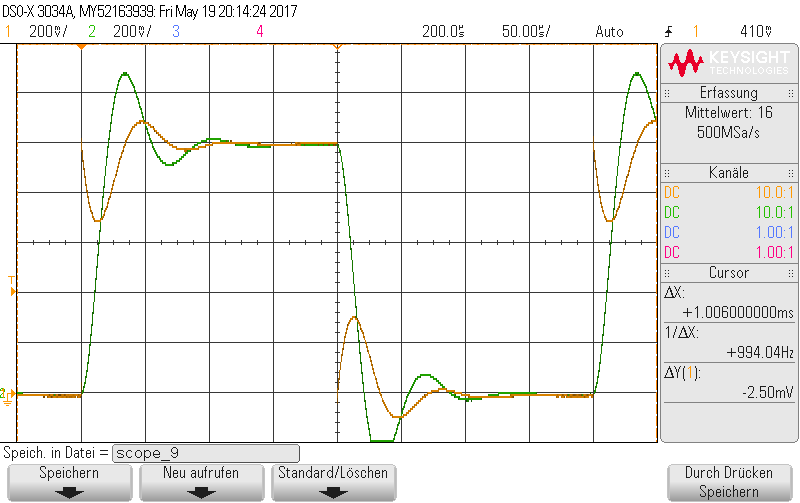
\includegraphics[width=1\textwidth]{./Oszi_Bilder/RLC_Sprung_22.png}
    \caption{Sprungantwort mit $R=22\Omega$, $U_e$ (gelb), $U_a$ (gr\"un)}
  \end{center}
\end{figure}
\noindent
Bereits in der Sprungantwort ist zu erkennen, dass das System mit einem Widerstand von nur $22\Omega$ \"uberschwingen wird, da die Ausgangsspannung an den Flanken stark \"uberschwingt. Die Schwingungen an der Eingangsspannung werden durch die Induktivität der Spule verursacht.

\subsection{Bodediagramm $R=22\Omega$}

\begin{figure}[H]
  \centering
  \begin{tikzpicture}
    \begin{axis}[width=15cm, height=7cm, xmode=log, xmin=10, xmax=1e7, xlabel={Frequenz [Hz]}, ylabel={Amplitude [dB]},y tick label style={grid=major}]
      \addplot table[x=Frequenz, y=dB, col sep=comma] {./csv_files/RLC_22_amplitude.csv};
      %\node[label={260:{$f_g$}},circle,fill=black,inner sep=3pt] at (axis cs:15580,12) {};
    \end{axis}
  \end{tikzpicture}
  \caption{Bode Diagramm RLC-Tiefpass, $R=22\Omega$, Amplitudengang}
\end{figure}
\begin{figure}[H]
  \centering
  \begin{tikzpicture}
    \begin{axis}[width=15cm, height=7cm, xmode=log, xmin=10, xmax=1e7, xlabel={Frequenz [Hz]}, ylabel={Phase [$^\circ$]},y tick label style={grid=major}]
      \addplot table[x=Frequenz, y=Phase, col sep=comma] {./csv_files/RLC_22_phase.csv};
      %\node[label={260:{$f_g$}},circle,fill=black,inner sep=3pt] at (axis cs:15580,12) {};
    \end{axis}
  \end{tikzpicture}
  \caption{Bode Diagramm RLC-Tiefpass, $R=22\Omega$, Phasengang}
\end{figure}
\noindent
Da es sich bei dieser Messung um einen Tiefpass handelt is die D\"ampfung bis zur Grenzfrequenz 0dB und das Eingangsignal wird unver\"andert durchgelassen. Wie bereits in der Sprungantwort festgestellt schwingt der Filter genau bei der Grenzfrequenz, das heißt die Ausgangsspannung ist gr\"o\ss{}er als die Eingangspannung. Danach beginnt der Fiter mit $-40dB/Dec$ zu d\"ampfen. Die Phase dreht von $0^\circ$ auf $-180^\circ$, genau bei der Grenzfrequenz beträgt der Phasenwinkel $-90^\circ$. \\
Die letzten 5 Messpunkte sind sehr ungenau, da das Ausgangssignal bereits so stark ged\"ampft ist, dass keine genauen Messungen mehr durchgef\"uhrt werden konnten. \\ \\
Die genaue Grenzfrequenz sollte mittels Variation der Frequenz am Funktionsgenerator festgestellt werden. Dabei wird die Frequenz so lange erh\"oht bis die Phasenverschiebung genau $-90^\circ$ betr\"agt. \\ \\
Ermittelte Grenzfrequenz: $f_0=15580Hz$ \\ \\
Berechnete Grenzfrequenz: $f_0=\frac{1}{2\pi * \sqrt{LC}}=\frac{1}{2\pi * \sqrt{100nF*1mH}} = 15916Hz$ \\ \\
Unterschied zwischen berechneten und gemessenen Wert: $2,11\%$.


\subsection{Sprungantwort $R=180\Omega$}

\begin{figure}[H]
  \begin{center}
    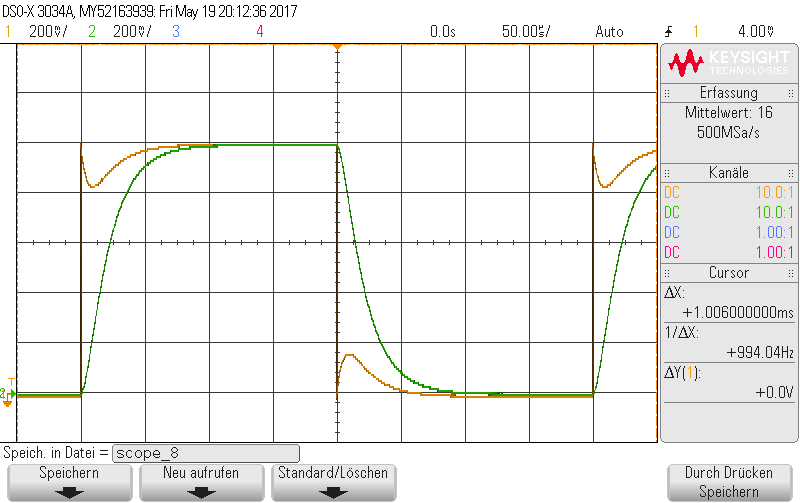
\includegraphics[width=1\textwidth]{./Oszi_Bilder/RLC_Sprung_180.png}
    \caption{Sprungantwort mit $R=180\Omega$, $U_e$ (gelb), $U_a$ (gr\"un)}
  \end{center}
\end{figure}
\noindent
Mit dem gr\"o\ss{}eren Widerstand, steigt die Ausgangsspannung reltativ schnell an, es kommt jedoch nicht zu \"uberschwingungen $\Rightarrow$ Filter kritisch ged\"ampft. \\

\subsection{Bodediagramm $R=180\Omega$}

\begin{figure}[H]
  \centering
  \begin{tikzpicture}
    \begin{axis}[width=15cm, height=7cm, xmode=log, xmin=10, xmax=1e7, xlabel={Frequenz [Hz]}, ylabel={Amplitude [dB]},y tick label style={grid=major}]
      \addplot table[x=Frequenz, y=dB, col sep=comma] {./csv_files/RLC_180_amplitude.csv};
      %\node[label={260:{$f_g$}},circle,fill=black,inner sep=3pt] at (axis cs:15580,12) {};
    \end{axis}
  \end{tikzpicture}
  \caption{Bode Diagramm RLC-Tiefpass, $R=180\Omega$, Amplitudengang}
\end{figure}
\begin{figure}[H]
  \centering
  \begin{tikzpicture}
    \begin{axis}[width=15cm, height=7cm, xmode=log, xmin=10, xmax=1e7, xlabel={Frequenz [Hz]}, ylabel={Phase [$^\circ$]},y tick label style={grid=major}]
      \addplot table[x=Frequenz, y=Phase, col sep=comma] {./csv_files/RLC_180_phase.csv};
      %\node[label={260:{$f_g$}},circle,fill=black,inner sep=3pt] at (axis cs:15580,12) {};
    \end{axis}
  \end{tikzpicture}
  \caption{Bode Diagramm RLC-Tiefpass, $R=180\Omega$, Phasengang}
\end{figure}
Da es sich hier um einen Filter mit kritischer D\"ampfung handelt, beginnt die D\"ampfung, kurz vor der Grenzfrequenz. Bei $-90^\circ$ Phasenverschiebung wurde eine D\"ampfung von -5dB gemessen. Ab der Grenzfrequenz beträgt die Filtersteilheit $-40dB/Dec$.

\subsection{Sprungantwort $R=1k\Omega$}

\begin{figure}[H]
  \begin{center}
    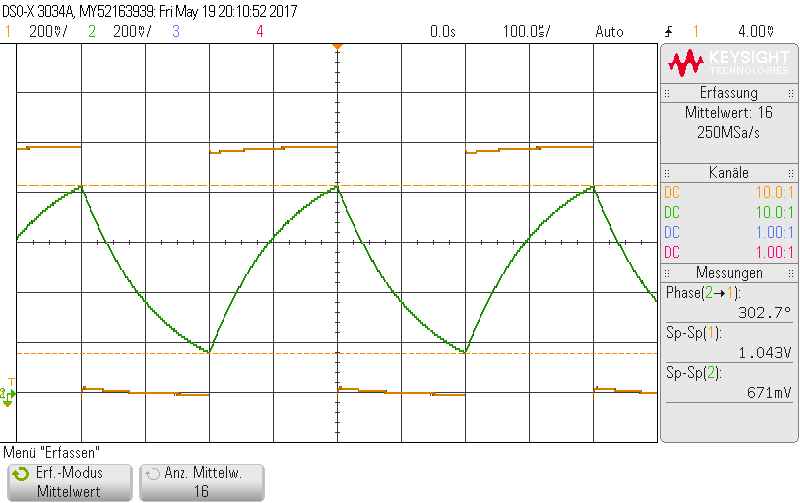
\includegraphics[width=1\textwidth]{./Oszi_Bilder/RLC_Sprung_1k.png}
    \caption{Sprungantwort mit $R=1k\Omega$, $U_e$ (gelb), $U_a$ (gr\"un)}
  \end{center}
\end{figure}
\noindent
Mit einem gro\ss{}en Widerstand von $R=1k\Omega$ ist die Zeitkonstante $\tau$ sehr gro\ss{}, d.h. der Filter braucht sehr lange bis der Endwert erreicht wird.

\subsection{Bodediagramm $R=1k\Omega$}

\begin{figure}[H]
  \centering
  \begin{tikzpicture}
    \begin{axis}[width=15cm, height=7cm, xmode=log, xmin=10, xmax=1e7, xlabel={Frequenz[Hz]}, ylabel={Amplitude [dB]},y tick label style={grid=major}]
      \addplot table[x=Frequenz, y=dB, col sep=comma] {./csv_files/RLC_1k_amplitude.csv};
      %\node[label={260:{$f_g$}},circle,fill=black,inner sep=3pt] at (axis cs:15580,12) {};
    \end{axis}
  \end{tikzpicture}
  \caption{Bode Diagramm RLC-Tiefpass, $R=1k\Omega$, Amplitudengang}
\end{figure}
\begin{figure}[H]
  \centering
  \begin{tikzpicture}
    \begin{axis}[width=15cm, height=7cm, xmode=log, xmin=10, xmax=1e7, xlabel={Frequenz [Hz]}, ylabel={Phase [$^\circ$]},y tick label style={grid=major}]
      \addplot table[x=Frequenz, y=Phase, col sep=comma] {./csv_files/RLC_1k_phase.csv};
      %\node[label={260:{$f_g$}},circle,fill=black,inner sep=3pt] at (axis cs:15580,12) {};
    \end{axis}
  \end{tikzpicture}
  \caption{Bode Diagramm RLC-Tiefpass, $R=1k\Omega$, Phasengang}
\end{figure}
Dieses schlechte D\"ampfungsverhalten, welches bereits in der Sprunganwort zu erkenne war, zeichnet sich auch im Bodediagramm ab. Der Filter beginnt bereits sehr fr\"uh zu d\"ampfen, jedoch betr\"agt die Filtersteilheit nur -20dB/Dec. Dies liegt daran, dass nur der RC-Teil aktiv ist. Die Grenzfrequenz des RL-Teils liegt weit dar\"uber, bei ca. $150kHz$. Dieser Knick ist allerdings im Amplitudengang nur mehr sehr schlecht zu erkennen, da bei dieser hohen Frequenz das Ausgangsignal beretis so stark ged\"ampft wurde, dass keine vern\"uftigen Messergebnisse mehr aufgenommen werden konnten. Im Phasengang, ist die Drehung von $-90^\circ$ auf $-180^\circ$ bei ca. $150kHz$ zu erkennen. \\ \\
Grenzfrequenz des RC-Teiles: $f_g=\frac{1}{2\pi RC}=\frac{1}{2\pi*1k\Omega *100nF}=1591Hz$ \\ \\
Grenzfrequenz des LC-Teiles: $f_g=\frac{R}{2\pi L} = \frac{1k\Omega}{2\pi*1mH}=159155Hz$

\subsection{Pol- Nullstellendiagramm}

\begin{figure}[H]
  \begin{center}
    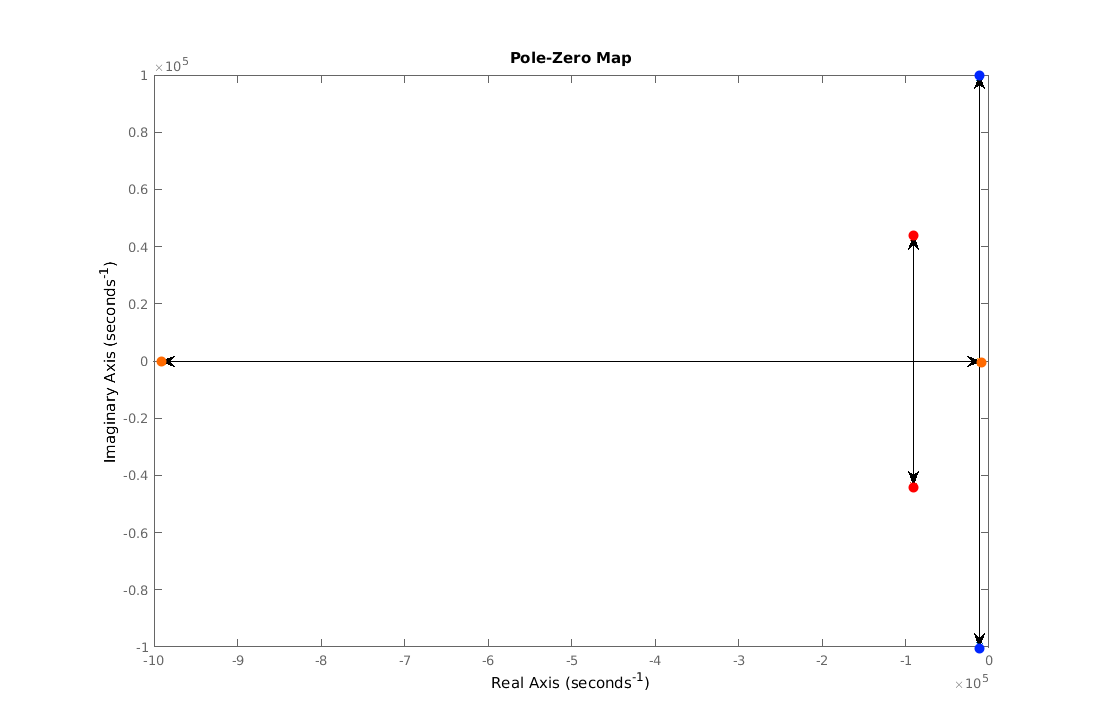
\includegraphics[width=1\textwidth]{./PoleZeroMap.png}
    \caption{Pol- Nullstellen Diagramm}
  \end{center}
\end{figure}
\noindent
Das Diagramm zeigt die Polstellen der verschiedenen Messungen. Die orangen Punkte, mit Imaginärwert 0, sind vom $1k\Omega$ Widerstand, die roten Punkte, bei $40kHz$, vom $180\Omega$ Widerstand und die
blauen Punkte, Realwert 0, sind vom $22\Omega$ Widerstand.

\subsection{Vergleich: Messung und Simulationen}
Die Messungen stimmen bis auf kleine Bauteil- und Messungenauigkeiten mit den Simulationen \"uberein. \\
Die Messungen der Ausgangssingale im hochfrequenten Bereich ($>100kHz$) sind im Vergleich zu den Simulationen sehr ungenau, da das Signal bereits zu stark ged\"ampft ist. \newpage


\end{document}
